\documentclass[conference]{IEEEtran}
\usepackage{graphicx}
\usepackage{mathtools}
\usepackage{multirow}
\usepackage[justification=centering]{caption}
\usepackage{amsmath}
\usepackage{float}
\usepackage[table]{xcolor}
\usepackage[linesnumbered,ruled,vlined]{algorithm2e}
\usepackage{algpseudocode}
\usepackage{cite}
\usepackage{subcaption}
\captionsetup{font=small}
\graphicspath{}
\DeclareGraphicsExtensions{.jpg,.png}
\usepackage{fancyhdr,lipsum}
\usepackage{kantlipsum}
\newcommand\tab[1][0.5cm]{\hspace*{#1}}
\usepackage{hyperref}




\pagestyle{plain}
\setcounter{page}{469}


\begin{document}

\title{\LARGE Constraint Satisfaction Problem(CSP) \\Comparative Performance Analysis of Arc-Consistency Algorithms\\AC-1, AC-2, AC-3, AC4}
\author
{	Amit Roy, Roll: JH-40
	\\Department of Computer Science and Engineering,\\University of Dhaka,\\Email: \href{mailto:aroy7298@gmail.com}{aroy7298@gmail.com}
}
\maketitle
\section{Problem Definition}
\label{Introduction}
\fontsize{9.9pt}{9.9pt}\selectfont\noindent
Artificial intelligence tasks can be formulated as \textbf{Constraint Satisfaction Problems(CSP)}.Constraint satisfaction problem consists of three components, $\langle$ \textbf{\textit{X,D,C}}$\rangle$\\
\tab\textbf{X:} A set of variables, \textbf{\{X$_1$, . . . , X$_n$\}}.\\
\tab\textbf{D:} A set of domains, \textbf{\{D$_1$, . . . , D$_n$\}}, one for each variable.\\
\tab\textbf{C:} A set of constraints that specify allowable 
\tab combinations of values.\\
Each domain \textbf{D$_i$} consists of a set of allowable values, \textbf{\{v$_1$, . . . ,v$_n$\}} for each variable \textbf{X$_i$}. Each constraint \textbf{C$_i$} consists of a relation between two variables. This type of constraint is called \textbf{binary constraint}.\\\noindent
\noindent An assignment that does not violate any constraints is called a \textbf{consistent} or \textbf{legal assignment}. A \textbf{complete assignment} is one in which every variable is assigned, and a solution to a CSP is a \textbf{consistent, complete assignment}.\\
\noindent Before making an attempt to construct a complete solution of a CSP problem, we should eliminate local inconsistencies. A variable in a CSP is \textbf{arc-consistent} if every value in its domain satisfies the variable's binary constraints.\\
\noindent \textbf{X$_i$} is arc-consistent with respect to another variable \textbf{X$_j$} if for every value in the current domain \textbf{D$_i$} there is some value in the domain \textbf{D$_j$} that satisfies the binary constraint on the arc $\bf{\left(X_{i},X_{j}\right)}$. A network is arc-consistent if every variable is arc-consistent with every other variable.\\
\noindent In this problem we wish to implement the most popular algorithms for arc-consistency named AC-1, AC-2, AC-3, AC4.
	\begin{figure}[h]
	\centering
			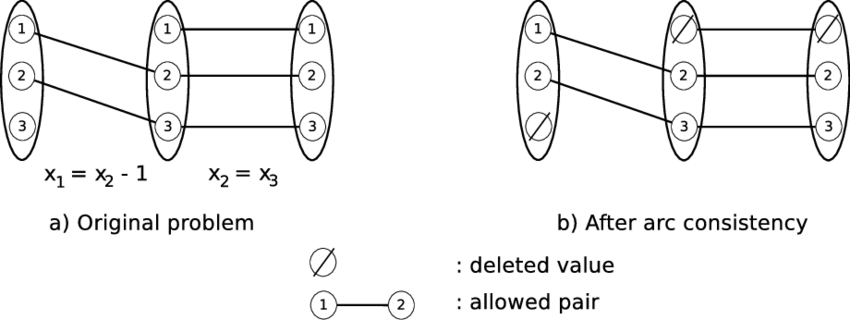
\includegraphics[width=6cm]{pic2.png}
			\captionsetup{singlelinecheck = false, format= hang,  font=footnotesize, labelsep=space}
			\caption{Example of Binary CSP}
\end{figure}
\section{Constraints}\noindent To implement the arc-consistency algorithms we need a set of constraints which will contain some relations between two variables of the consistency graph. For the sake of simplicity we are considering binary constraints between two variables and we define a set of mathematical relations as the constraints.\\\textbf{Constraints:}
\begin{equation}
y \leq x
\end{equation}
\begin{equation}
y \geq x
\end{equation}
\begin{equation}
y=x
\end{equation}
\begin{equation}
y \neq x
\end{equation}
\begin{equation}
y\%x=0 \mbox{, y divides x}
\end{equation}
\begin{equation}
gcd(x,y)=1 \mbox{ i.e. x and y are co-prime}
\end{equation}
\begin{equation}
y=mx + c \mbox{, m and c are constant}
\end{equation}
\begin{equation}
y=ax^2 + bx + c \mbox{, a,b and c are constant}
\end{equation}
\noindent Before implementing an arc-consistency algorithm, we will generate random graph for different number of nodes(e.g 5,10,15,20) of the network using some built library(e.g. NetworkX in python). Then, for each edge of the network we will randomly choose a constraint from the predefined constraints list and then assign that constraint on that particular arc.\\
\noindent We use those constraints to check the consistency of the nodes. Suppose two node \textbf{X$_i$} and \textbf{X$_j$} share an arc between them in the network. While checking whether \textbf{X$_i$} is arc-consistent with respect to \textbf{X$_j$}, we will check for every value x $\in$ \textbf{D$_i$}, whether there is a corresponding value y $\in$ \textbf{D$_j$} which satisfies the constraint assigned on the arc between \textbf{X$_i$} and \textbf{X$_j$}. If x $\notin$ \textbf{D$_i$} then x is removed from \textbf{D$_i$} to make it arc-consistent with respect to \textbf{X$_j$}
\section{Domains}\noindent
As we have already defined, a CSP problem has a set of domains, one for each variable. Since our constraints are mathematical equations we will choose integers within a range as the domain.
\\For each variable, first we will randomly choose a domain size within a range(e.g. 20-100). When the domain size of a variable is fixed, we will assign values to the domain of that variable. While assigning we can choose a range between 1 and 10000 and pick values randomly from this range as the domain of that variable.
\\Those domains will be necessary to determine whether two variables sharing an arc between them satisfy the constraint of that arc. In other words, the purpose of these domains of each variable is to check the arc-consistency between two variables.
\section{Comparative Performance Analysis}
\noindent After generating the graph, assigning constraining on the edges and and also defining the domains of each variable we will run the \textbf{AC-1,AC-2,AC-3,AC-4} algorithms on the network. For the same number of nodes we will generate different graphs and run the algorithms several(10-20) times on them and take the average value of the performance metrics(e.g. running time or \% of domain reduction per edge).\\
\noindent Finally we will plot a graph where the \textbf{Y axis} will be \textbf{performance metrics} and \textbf{X axis} will be \textbf{number of nodes} in the network. We can find 4 lines for four different algorithms and compare between them by analyzing the graph.

\end{document}

